\documentclass[a4paper]{article}
\usepackage[a4paper,margin=0mm]{geometry}
\usepackage{fontspec}
\usepackage{unicode-math}
\usepackage{tikz}
\usepackage[table]{xcolor}
\usepackage[absolute]{textpos}
\usepackage{enumitem}
\usepackage{array}
\usepackage{multirow}

\setmainfont{Libertinus Serif}
\setsansfont{Libertinus Sans}
\setmathfont{Libertinus Math}
\newfontfamily\trackedsans{Libertinus Sans}[LetterSpace=8.0]

\definecolor{accent}{HTML}{602785}
\definecolor{badge}{HTML}{B8A0C8}
\definecolor{ink}{HTML}{2A2E30}

\setlength{\TPHorizModule}{1mm}
\setlength{\TPVertModule}{1mm}
\setlength{\parindent}{0pt}
\pagestyle{empty}

\newcommand{\LCOL}{16mm}
\newcommand{\RCOL}{111mm}
\newcommand{\COLW}{83mm}

\newcommand{\topicheader}[2]{%
\begin{textblock*}{194mm}(16mm,10mm)
\begin{tikzpicture}
\node[fill=accent,text=white,font=\sffamily\bfseries\fontsize{13}{13}\selectfont,
      minimum width=9mm,minimum height=9mm,inner sep=0pt] at (4.5mm,-4.5mm) {#1};
\node[font=\sffamily\bfseries\fontsize{15}{16}\selectfont,text=ink,anchor=west] at (12mm,-4.5mm) {#2};
\end{tikzpicture}
\end{textblock*}
\begin{textblock*}{194mm}(16mm,22.5mm)

\begin{tikzpicture}
\fill[accent] (0,0) rectangle (194mm,0.5mm);
\end{tikzpicture}
\end{textblock*}
}

\newcommand{\pagefooter}[1]{%
\begin{textblock*}{194mm}(8mm,286.41mm)
  
\begin{tikzpicture}
    \fill[accent] (0,0) rectangle (194mm,0.6mm);
  \end{tikzpicture}
\end{textblock*}
\begin{textblock*}{63.59mm}(8mm,288.27mm)
  {\sffamily\bfseries\color{accent}\fontsize{13}{16}\selectfont SAT 1200+}
\end{textblock*}
\begin{textblock*}{10mm}(188mm,288.27mm)
  \centering{\sffamily\color{accent}\fontsize{14}{16}\selectfont #1}
\end{textblock*}
}

\newcommand{\colrule}[2]{%
\begin{textblock*}{1mm}(105mm,#1mm)
\begin{tikzpicture}
\draw[black!65,line width=0.5pt] (0,0) -- (0,#2mm);
\end{tikzpicture}
\end{textblock*}
}

\newcommand{\setkicker}[2]{%
{\sffamily\bfseries\fontsize{12}{14}\selectfont #1.}\ {\itshape\fontsize{11}{14}\selectfont\color{black!75} #2}\par\vspace{2mm}%
}

\setlength{\fboxsep}{1.4pt}
\setlength{\fboxrule}{0.5pt}
\newcommand{\pnum}[1]{\fcolorbox{ink}{white}{\sffamily\bfseries\fontsize{8}{8}\selectfont #1}~}

\newcommand{\qrbox}[1]{%
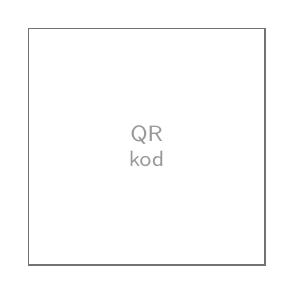
\begin{tikzpicture}
\draw[black!55,line width=0.6pt] (0,0) rectangle (30mm,30mm);
\node[black!40,font=\sffamily\fontsize{8}{9}\selectfont,align=center] at (15mm,15mm) {QR\\kod};
\end{tikzpicture}\\[1.5mm]
{\sffamily\fontsize{9}{11}\selectfont\color{black!70} #1}%
}

\arrayrulecolor{accent}
\setlength{\arrayrulewidth}{0.7pt}
\renewcommand{\arraystretch}{1.35}
\newcommand{\anstitle}[1]{{\sffamily\bfseries\color{accent}\fontsize{11}{13}\selectfont #1}\\[1.3mm]}

\begin{document}

% ================= PAGE 1: Set 1 | Set 2 =================
\topicheader{21}{Aylana}
\pagefooter{113}
\colrule{32}{238}
\mbox{}%

\begin{textblock*}{\COLW}(\LCOL,32mm)
{\fontsize{10.5}{13.5}\selectfont
\setkicker{1-to'plam}{Yoy uzunligi -- radius va markaziy burchak berilgan yoki izlanadi.}

\noindent\pnum{1} Radiusi $9$ sm, markaziy burchak $40°$. Yoy uzunligini toping.\\[14mm]
\noindent\pnum{2} Radiusi $15$ sm, markaziy burchak $72°$. Yoy uzunligini toping.\\[14mm]
\noindent\pnum{3} Radiusi $8$ sm, markaziy burchak $270°$. Yoy uzunligini toping.\\[14mm]
\noindent\pnum{4} Radiusi $6$ sm, yoy uzunligi $4\pi$ sm. Markaziy burchakni (daraja) toping.\\[14mm]
\noindent\pnum{5} Radiusi $10$ sm, yoy uzunligi $5\pi$ sm. Markaziy burchakni toping.\\[14mm]
\noindent\pnum{6} Yoyning markaziy burchagi $50°$. Yoy o'lchovi nechaga teng? Uzunlikni topish uchun yana qanday ma'lumot kerak?
}
\end{textblock*}

\begin{textblock*}{\COLW}(\RCOL,32mm)
{\fontsize{10.5}{13.5}\selectfont
\setkicker{2-to'plam}{Sektor yuzi -- radius va markaziy burchak berilgan yoki izlanadi.}

\noindent\pnum{1} Radiusi $6$ sm, markaziy burchak $60°$. Sektor yuzini toping.\\[14mm]
\noindent\pnum{2} Radiusi $12$ sm, markaziy burchak $150°$. Sektor yuzini toping.\\[14mm]
\noindent\pnum{3} Radiusi $9$ sm, markaziy burchak $40°$. Sektor yuzini toping.\\[14mm]
\noindent\pnum{4} Radiusi $20$ sm, markaziy burchak $18°$. Sektor yuzini toping.\\[14mm]
\noindent\pnum{5} Radiusi $10$ sm, sektor yuzi $15\pi$ sm². Markaziy burchakni toping.\\[14mm]
\noindent\pnum{6} Radiusi $18$ sm, sektor yuzi $27\pi$ sm². Markaziy burchakni toping.
}
\end{textblock*}

\clearpage

% ================= PAGE 2: Set 3 | Set 4 =================
\topicheader{21}{Aylana}
\pagefooter{114}
\colrule{32}{238}
\mbox{}%

\begin{textblock*}{\COLW}(\LCOL,32mm)
{\fontsize{10.5}{13.5}\selectfont
\setkicker{3-to'plam}{Aralash: yoy uzunligi va sektor yuzi -- bitta doira, bitta burchak. Ikkalasini aralashtirmang.}

\noindent\pnum{1} Radiusi $6$ sm, markaziy burchak $90°$. Yoy \textbf{uzunligini} toping.\\[12mm]
\noindent\pnum{2} (Yuqoridagi doira, xuddi shu burchak.) Sektor \textbf{yuzini} toping.\\[12mm]
\noindent\pnum{3} Radiusi $9$ sm, markaziy burchak $200°$. Yoy \textbf{uzunligini} toping.\\[12mm]
\noindent\pnum{4} (Yuqoridagi doira, xuddi shu burchak.) Sektor \textbf{yuzini} toping.\\[12mm]
\noindent\pnum{5} Purkagich radiusi $18$ fut bo'lgan maydonni $50°$ markaziy burchak bo'yicha sug'oradi. Purkagich uchi chizadigan yoyning uzunligini toping.\\[14mm]
\noindent\pnum{6} Xuddi shu purkagich sug'oradigan maydonning (sektor) yuzini toping.
}
\end{textblock*}

\begin{textblock*}{\COLW}(\RCOL,32mm)
{\fontsize{11}{14}\selectfont
\setkicker{4-to'plam}{Markaz $(h,k)$ va radius $r$ ni toping.}

\noindent\pnum{1} $(x-2)^2+(y-5)^2=49$\\[20mm]
\noindent\pnum{2} $(x+3)^2+(y-1)^2=16$\\[20mm]
\noindent\pnum{3} $(x-7)^2+(y+6)^2=81$\\[20mm]
\noindent\pnum{4} $x^2+(y-4)^2=25$\\[20mm]
\noindent\pnum{5} $(x+1)^2+(y+1)^2=2$\\[20mm]
\noindent\pnum{6} $(x-5)^2+y^2=25$
}
\end{textblock*}

\clearpage

% ================= PAGE 3: Set 5 | Set 6 (spot the error) =================
\topicheader{21}{Aylana}
\pagefooter{115}
\colrule{32}{238}
\mbox{}%

\begin{textblock*}{\COLW}(\LCOL,32mm)
{\fontsize{11}{14}\selectfont
\setkicker{5-to'plam}{To'liq kvadratga keltiring: $(x-h)^2+(y-k)^2=r^2$. Markaz va radiusni toping.}

\noindent\pnum{1} $x^2+y^2-4x-6y-12=0$\\[18mm]
\noindent\pnum{2} $x^2+y^2+10x-4y+13=0$\\[18mm]
\noindent\pnum{3} $x^2+y^2-2x+8y+1=0$\\[18mm]
\noindent\pnum{4} $x^2+y^2+6x+6y+9=0$\\[18mm]
\noindent\pnum{5} $x^2+y^2-8x+2y-8=0$\\[18mm]
\noindent\pnum{6} $x^2+y^2+2x-12y+12=0$
}
\end{textblock*}

\begin{textblock*}{\COLW}(\RCOL,32mm)
{\fontsize{10}{13}\selectfont
\setkicker{6-to'plam}{Xatoni toping -- buzilgan qadamni ayting, to'g'ri javobni bering.}

\noindent\pnum{1} Radiusi $9$ sm, markaziy burchak $40°$ bo'lgan yoyning uzunligini toping.\\[1mm]
\hspace*{7mm}\textit{``Yoy uzunligi $=40$ sm.''}\\[2mm]
\hspace*{7mm}Xato va to'g'ri javob: \makebox[50mm]{\dotfill}\\[6mm]

\noindent\pnum{2} Radiusi $10$ sm, markaziy burchak $90°$ bo'lgan sektorning yuzini toping.\\[1mm]
\hspace*{7mm}\textit{``Sektor yuzi $=\frac{90}{360}\times2\pi\times10=5\pi$ sm².''}\\[2mm]
\hspace*{7mm}Xato va to'g'ri javob: \makebox[50mm]{\dotfill}\\[6mm]

\noindent\pnum{3} $x^2+y^2-10x+4y-7=0$ markazi va radiusini toping.\\[1mm]
\hspace*{7mm}\textit{``$(x^2-10x)+(y^2+4y)=-7$, $(x-5)^2+(y+2)^2=-7+25+4=22$.''}\\[2mm]
\hspace*{7mm}Xato va to'g'ri javob: \makebox[50mm]{\dotfill}\\[6mm]

\noindent\pnum{4} $(x+6)^2+(y-3)^2=49$ markazini toping.\\[1mm]
\hspace*{7mm}\textit{``Markaz $(6,3)$.''}\\[2mm]
\hspace*{7mm}Xato va to'g'ri javob: \makebox[50mm]{\dotfill}\\[6mm]

\noindent\pnum{5} Radiusi $16$ sm, yoy uzunligi $8\pi$ sm. Markaziy burchakni toping.\\[1mm]
\hspace*{7mm}\textit{``$8\pi=\frac{\theta}{360}\times\pi\times16^2$, bundan $\theta$ ni topamiz.''}\\[2mm]
\hspace*{7mm}Xato va to'g'ri javob: \makebox[50mm]{\dotfill}
}
\end{textblock*}

\clearpage

% ================= PAGE 4: Set 7 (bonus) -- own page =================
\topicheader{21}{Aylana}
\pagefooter{116}
\colrule{32}{238}
\mbox{}%

\begin{textblock*}{\COLW}(\LCOL,32mm)
{\fontsize{10.5}{13.5}\selectfont
\setkicker{7-to'plam}{Bonus / qiyin.}

\noindent\pnum{1} Sektorning yuzi $24\pi$ sm², markaziy burchagi $60°$. Doiraning radiusini toping.\\[20mm]
\noindent\pnum{2} Yoyning uzunligi $10\pi$ sm, markaziy burchagi $100°$. Avval radiusni, so'ngra xuddi shu burchak uchun sektor yuzini toping.\\[22mm]
\noindent\pnum{3} $x^2+y^2-14x-8y+40=0$. Markaz va radiusni toping, so'ngra $(7,4)$ nuqtasi doira ichida, tashqarisida, yoki aylananing ustida ekanligini aniqlang.\\[26mm]
\noindent\pnum{4} Sektorning yuzi to'liq doira yuzining $\dfrac{1}{8}$ qismi. Markaziy burchakni toping. Agar radius $16$ sm bo'lsa, yoy uzunligini toping.\\[22mm]
\noindent\pnum{5} $x^2+y^2+4x-10y-20=0$. Markaz va radiusni toping. So'ngra markaziy burchagi $72°$ bo'lgan sektorning yoy uzunligi va yuzini toping.
}
\end{textblock*}

\clearpage

% ================= PAGE 5: Javoblar =================
\topicheader{21}{Aylana}
\pagefooter{117}
\mbox{}%

\begin{textblock*}{194mm}(16mm,30mm)
{\bfseries\itshape\color{accent}\fontsize{19}{21}\selectfont\centering Javoblar\par}
\end{textblock*}

\begin{textblock*}{194mm}(16mm,44mm)
{\fontsize{9}{11.5}\selectfont
\centering
\renewcommand{\arraystretch}{1.3}
\begin{tabular}{|>{\centering\arraybackslash}p{24mm}|>{\centering\arraybackslash}p{9mm}|>{\centering\arraybackslash}p{40mm}|>{\centering\arraybackslash}p{9mm}|>{\centering\arraybackslash}p{40mm}|}
\hline
\rowcolor{badge!55}\textbf{To'plam} & \textbf{\#} & \textbf{Javob} & \textbf{\#} & \textbf{Javob}\\
\hline
\multirow{3}{24mm}{\centering 1-to'plam} & 1 & $2\pi$ sm & 2 & $6\pi$ sm\\\cline{2-5}
 & 3 & $12\pi$ sm & 4 & $120°$\\\cline{2-5}
 & 5 & $90°$ & 6 & o'lchov $50°$; uzunlik uchun radius kerak\\\hline
\multirow{3}{24mm}{\centering 2-to'plam} & 1 & $6\pi$ sm² & 2 & $60\pi$ sm²\\\cline{2-5}
 & 3 & $9\pi$ sm² & 4 & $20\pi$ sm²\\\cline{2-5}
 & 5 & $54°$ & 6 & $30°$\\\hline
\multirow{3}{24mm}{\centering 3-to'plam} & 1 & $3\pi$ ft & 2 & $9\pi$ sm²\\\cline{2-5}
 & 3 & $10\pi$ sm & 4 & $45\pi$ sm²\\\cline{2-5}
 & 5 & $5\pi$ fut & 6 & $45\pi$ fut²\\\hline
\multirow{3}{24mm}{\centering 4-to'plam} & 1 & $(2,5)$, $r{=}7$ & 2 & $(-3,1)$, $r{=}4$\\\cline{2-5}
 & 3 & $(7,-6)$, $r{=}9$ & 4 & $(0,4)$, $r{=}5$\\\cline{2-5}
 & 5 & $(-1,-1)$, $r{=}\sqrt2$ & 6 & $(5,0)$, $r{=}5$\\\hline
\multirow{3}{24mm}{\centering 5-to'plam} & 1 & $(2,3)$, $r{=}5$ & 2 & $(-5,2)$, $r{=}4$\\\cline{2-5}
 & 3 & $(1,-4)$, $r{=}4$ & 4 & $(-3,-3)$, $r{=}3$\\\cline{2-5}
 & 5 & $(4,-1)$, $r{=}5$ & 6 & $(-1,6)$, $r{=}5$\\\hline
\multirow{5}{24mm}{\centering 6-to'plam} & \multicolumn{4}{p{92mm}|}{1.\ Yoy o'lchovini uzunlik deb yozgan. To'g'ri: $\frac{40}{360}\times2\pi\times9=2\pi$ sm.}\\\cline{2-5}
 & \multicolumn{4}{p{92mm}|}{2.\ Yuza o'rniga uzunlik formulasi qo'llangan. To'g'ri: $\frac{90}{360}\times\pi\times10^2=25\pi$ sm².}\\\cline{2-5}
 & \multicolumn{4}{p{92mm}|}{3.\ Erkin hadning ishorasi o'zgartirilmagan. To'g'ri: $(x-5)^2+(y+2)^2=36$; markaz $(5,-2)$, $r=6$.}\\\cline{2-5}
 & \multicolumn{4}{p{92mm}|}{4.\ $(x+6)^2$ ishorasi teskari o'qilgan. To'g'ri: markaz $(-6,3)$.}\\\cline{2-5}
 & \multicolumn{4}{p{92mm}|}{5.\ Uzunlik o'rniga yuza formulasi qo'llangan. To'g'ri: $8\pi=\frac{\theta}{360}\times2\pi\times16$, $\theta=90°$.}\\\hline
\multirow{5}{24mm}{\centering 7-to'plam} & \multicolumn{4}{p{92mm}|}{1.\ $r=12$ sm}\\\cline{2-5}
 & \multicolumn{4}{p{92mm}|}{2.\ $r=18$ sm; sektor yuzi $=90\pi$ sm²}\\\cline{2-5}
 & \multicolumn{4}{p{92mm}|}{3.\ Markaz $(7,4)$, $r=5$; nuqta aynan markaz -- doira ichida.}\\\cline{2-5}
 & \multicolumn{4}{p{92mm}|}{4.\ $\theta=45°$; yoy uzunligi $=4\pi$ sm}\\\cline{2-5}
 & \multicolumn{4}{p{92mm}|}{5.\ Markaz $(-2,5)$, $r=7$; yoy uzunligi $=\frac{14\pi}{5}$ sm, sektor yuzi $=\frac{49\pi}{5}$ sm²}\\\hline
\end{tabular}
}
\end{textblock*}

\begin{textblock*}{194mm}(16mm,220mm)
\centering
{\sffamily\fontsize{9.5}{11.5}\selectfont\color{black!70} Video yechimlar va qo'shimcha testlar uchun quyidagi QR kodlarni skanerlang:}\\[4mm]
\begin{minipage}[t]{32mm}\centering\qrbox{YouTube}\end{minipage}%
\hspace{16mm}%
\begin{minipage}[t]{32mm}\centering\qrbox{Telegram}\end{minipage}
\end{textblock*}

\end{document}
